\documentclass[11pt,a4paper]{article}

\usepackage[ngerman]{babel}
\usepackage[utf8]{inputenc}
\usepackage[T1]{fontenc}
\usepackage{lmodern}
\usepackage{amsmath}
\usepackage{graphicx}
\usepackage{float}
\usepackage{hyperref}

\title{Reinforcement Learning - Übung 01}
\author{Amos Mohr, Daniel Maier, Sifan Zhu, Tommy Kiss}
\date{\today}

\begin{document}

\maketitle

\section*{Übung 01}
Beobachtungen:
\begin{itemize}
    \item $\epsilon = 0$ entspricht reiner greedy-Auswahl in jedem Schritt, reward pro Schritt konvergiert knapp über 1
    \item $\epsilon = 1$ entspricht reiner exploration, daher ist Erwartungswert der Durchschnitt der Erwartungswerte der einzelnen arm-rewards. Diese sind normalverteilt um 0, somit Erwartung 0.
    \item Solange $\epsilon > 0$, findet Verfahren durch Exploration bessere Rewards als ohne Exploration.
    \item Für 1000 Schritte ist $\epsilon = 0.05$ aus unserer Auswahl am besten.
\end{itemize}
\section*{Übung 02}

\begin{figure}[H]
    \centering
    
\includegraphics[width=\textwidth]{plots/softmax.png}
    \caption{Durchschnittlicher Reward pro Schritt für Softmax, gemittelt über alle Experimente.}
    \label{fig:softmax-avg-reward}
\end{figure}

Man sieht: 0.1, 0.2 und 0.5 sind die besten drei Werte, der beste ist 0.2.
Die Werte 100 und 20 sind am schlechtesten.
Ab 1.0 fällt der reward pro step monoton mit steigendem Parameter.

\begin{figure}[H]
    \centering
    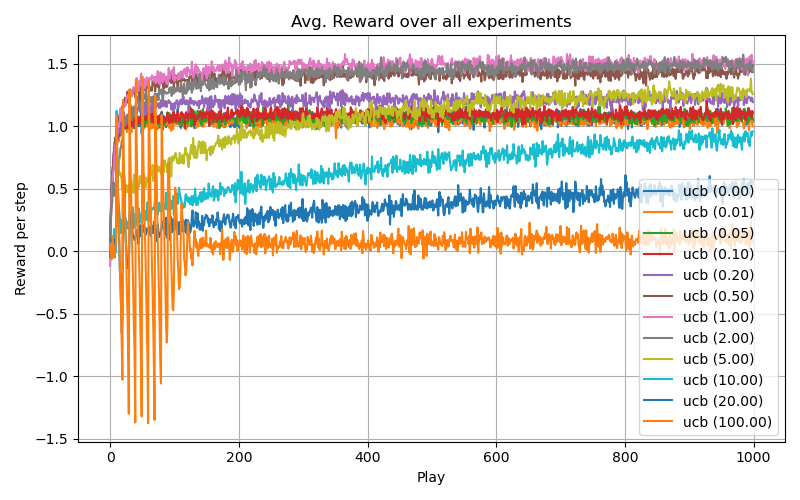
\includegraphics[width=\textwidth]{plots/ucb.png}
    \caption{Durchschnittlicher Reward pro Schritt für UCB, gemittelt über alle Experimente.}
    \label{fig:ucb-avg-reward}
\end{figure}
Man sieht: 0.5, 1.0 und 2.0 sind die besten drei Werte, der beste ist 1.0.
Die schlechtesten Werte sind 10.0, 20.0 und 100.0 wobei 100.0 mit Abstand am schlechtesten ist und auch die meisten Oszillationen hat.
Die Oszillationen sind nicht nur im 100er-Plot zu sehen, sondern beginnen schon bei 5.
Die Vermutung liegt nahe, dass durch höhere $c$-Werte die eigentliche Reward-Schätzung am Anfang in den Hintergrund rückt, und sich die Auswahl deshalb hauptsächlich aus dem Exploration-Term bestimmt.
Da dieser für jeden Arm mit der Auswahlanzahl des Arms schnell fällt, oszilliert das Verfahren am Anfang relativ deterministisch zwischen den einzelnen Armen, bis die Exploration-Terme klein genug werden, damit die Reward-Schätzung wieder dominiert.

\section*{Übung 03}
\begin{figure}[H]
    \centering
    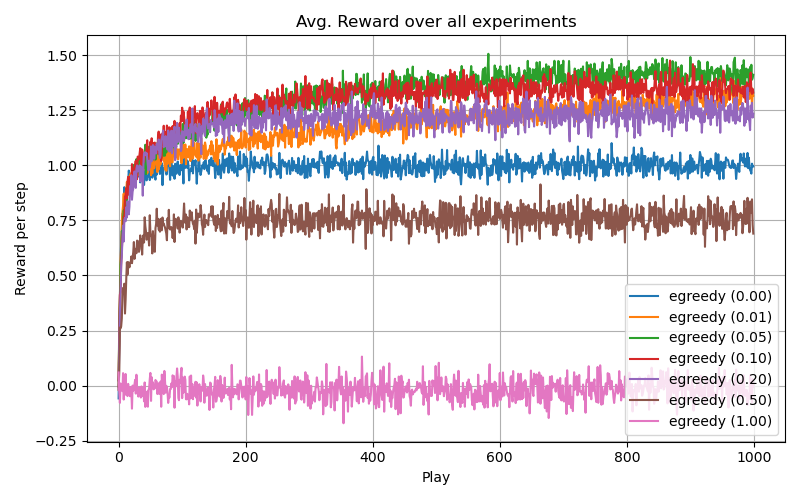
\includegraphics[width=\textwidth]{plots/egreedy.png}
    \caption{Durchschnittlicher Reward pro Schritt für $\epsilon$-greedy, gemittelt über alle Experimente.}
    \label{fig:egreedy-avg-reward}
\end{figure}

\begin{figure}[H]
    \centering
    
\includegraphics[width=\textwidth]{plots/custom.png}
    \caption{Durchschnittlicher Reward pro Schritt für exponentiell abfallendes $\epsilon$-greedy, gemittelt über alle Experimente.}
    \label{fig:custom-exp-decay-avg-reward}
\end{figure}
Das exponentiell abfallende $\epsilon$-greedy performt für sehr kleine $\epsilon$-Startwerte sehr ähnlich zu $\epsilon$-greedy.
Allerdings ist es viel konsistenter und ist sogar am besten mit den großen Werten, die für den nicht-exponentiellen $\epsilon$-greedy katastrophal sind.
Außerdem sind die besten Werte (0.5 und 1.0) konkurrenzfähig zu den besten UCB und Softmax-Werten, aber ohne die katastrophale Performance mit ungünstigen Werten und ohne Oszillationen.
Insgesamt kann man sagen dass diese Methode den besten Kompromiss aus Performance und Robustheit liefert.
\end{document}
